\documentclass[12pt]{article}

\usepackage[brazilian]{babel}
\usepackage[utf8]{inputenc}
\usepackage[a4paper, top = 3cm, left = 3cm, bottom = 2cm, right = 2cm]{geometry} 
\usepackage{amsmath} 
\usepackage{graphicx}
\usepackage{natbib}
\usepackage{indentfirst}
\usepackage{xcolor}

\graphicspath{ {Imagens/} }

\linespread{1.25} 

\title{Título do Trabalho}
\author{Nome do(a) Aluno(a) 1 \\
		Nome do(a) Aluno(a) 2 \\
		\textit{\small{Universidade Federal de Minas Gerais}}}
\date{29 de março de 2020}

\begin{document}
	
	\maketitle
	
	\section{Introdução} \label{sec:introducao}
	
	\par A introdução do texto tem a função de, principalmente, apresentar o problema que será estudado. Além disso, o(a) aluno(a) deve enunciar os motivos pelos quais a análise que será realizada é relevante.
	
	\par Essa seção \textbf{não} deve ser exageradamente grande. Em contrapartida, é importante que ela sirva de ``gancho'' para o leitor, fazendo com que ele tenha interesse em continuar com a leitura do trabalho.
	
	\section{Metodologia} \label{sec:metodologia}
	
	\par Aqui, devem ser apresentados os meios através dos quais o conjunto de dados foi obtido. 
	
	\par Em adição, os \textit{softwares} utilizados para análise da base de dados, bem como bibliotecas que estendem as funcionalidades padrão da linguagem de programação escolhida, devem ser mencionados.
	
	\section{Análise dos dados} \label{sec:analise}
	
	\par Essa é a parte mais importante do texto. Nessa seção, o(a) aluno(a) deverá utilizar os conceitos discutidos em sala para realizar uma análise pertinente dos dados. 
	
	\par A Análise Descritiva é \textbf{obrigatória}. Comentários que extrapolem esse tipo de estudo inicial não são necessários\footnote{Apesar disso, caso o(a) aluno(a) se sinta confortável em fazê-lo, não há problema.}.
	
	\par Para dar suporte aos argumentos apresentados, é \textbf{\color{red} necessário que gráficos e tabelas sejam incorporados ao texto}.
	
	\begin{figure}
		\centering
		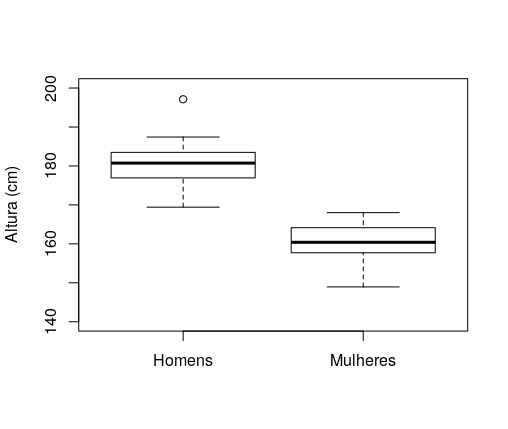
\includegraphics[width=.60\linewidth]{Boxplot}
		\vspace{-36pt}
		\caption{\small Boxplot para comparação de alturas (com $n = 100$ para cada grupo) entre Homens e Mulheres.}
		\label{fig:histograma}
	\end{figure}
	
	\par Aqui, pode acontecer de a Figura \ref{fig:histograma} não ser incorporada ao texto na mesma ordem em que ela foi incluída no código. Isso acontece porque o \LaTeX~determina, de maneira inteligente, o melhor lugar para posicionar a imagem (de modo que exista menos espaços em branco ao longo do documento).
	
	\begin{table}[h]
		\centering
		\begin{tabular}{c|c|c|c}
			\hline
			Classe (Idade) & $n_i$ & $f_i$ & $f_{ac}^{(i)}$ \\
			\hline \hline
			17 & 2 & 0.06 & 0.06 \\
			18 & 9 & 0.25 & 0.31 \\
			19 & 4 & 0.11 & 0.42 \\
			20 & 5 & 0.14 & 0.56 \\
			21 & 9 & 0.25 & 0.81 \\
			22 & 5 & 0.14 & 0.95 \\
			23 & 2 & 0.05 & 1.00 \\
			\hline \hline
			total & $n = 32$ & 1 & $-$ \\
			\hline
		\end{tabular}
		\caption{Tabela de frequência para conjunto de idades.}
		\label{tb:frequencia}
	\end{table}

	\par Depois de incluir a Tabela \ref{tb:frequencia}, é necessário explicá-la. Comentários pertinentes ao conteúdo que foi inserido devem \textbf{sempre} ser apresentados.
	
	\par Além disso, em adição às figuras, tabelas, etc., também é possível incluir fórmulas matemáticas, como a apresentada abaixo:
	
	\begin{equation}
		\bar{x} = \frac{1}{n}\sum_{i = 1}^{n}x_i.
	\end{equation}
	
	\par Não se esqueça de fazer referência às fontes utilizadas. Você pode escolher escrever algo como ``Segundo  \citet{magalhaes2002nocoes}, \textbf{amostra} é um subconjunto da população [$\cdots$]'', ou ``\textbf{Amostra} é um subconjunto da população \citep{magalhaes2002nocoes} [$\cdots$]''.
	
	\par Por fim, caso haja algum recurso que não foi mencionado ao longo desses curtos parágrafos, mas que seria interessante de ser adicionado à análise, sinta-se à vontade para fazer.
	
	\section{Comentários finais} \label{sec:final}
	
	\par Mais uma vez, essa seção deve ser breve (se comparada à Seção \ref{sec:analise}, principalmente). 
	
	\par Nessa última parte, devem ser listadas as conclusões finais sobre o trabalho e os pontos que ainda carecem de maior estudo e análise.
	
	\bibliographystyle{apa}
	\bibliography{Referencias/Referencias}
	
\end{document}